\section {Hologram emulation}
\label{sec.hologram_emulation}

The holographic display is a new generation of 3D display technology pursued by many researchers~\cite{Lucente1992, Watlington1995, Lucente2012} and companies~\cite{schwerdtner2013} over the past decades. Those works use special displays to create the hologram and they have in common a Spatial Light Modulator (SLM) in order tto create the incident source beam of light on the fringe pattern. The latter is generated by CGH and reflects the light beam,  but the necessary amount of data is not feasible for today's technology. For example, a 60-cm-diagonal hologram has a of over $10^{12}$ samples – the equivalent of a terabyte~\cite{Lucente2012}. While promising technologies have been proposed lately to decimate the amount of data~\cite{Lucente1992, schwerdtner2013}, there is a gap of the currently established 3D display technology and processing power for quality holograms. 

The proposal of this work is to investigate an emulation of holography using the 3D perception of standard stereo displays. The viewpoint is adjusted tracking the position of the viewer. One drawback is the restriction of a single viewer, but investigations to allow multiple viewers are still on pursuit~\cite{Frohlich2005}.

The cornerstone of the proposed projection is how this can be done with the existing viewing pipeline of 3D graphics frameworks such as OpenGL. 

The existing viewing transformations works well for 3D with positive stereo parallax, showing the object as inside the screen of display. In the opposite case, the projection with negative parallax requires the translation $T_{parallax}$ of the scene towards the virtual display. This is incorporated in the view transformation $M_{view}$ of Section~\ref{sec.projection_review}, creating a translated view $M_{view}T$. Let the modification of the viewpoint produce a new view transform $M^{\prime}_{view}$. This new viewpoint combined with $T_{parallax}$ is then defined as $M^{\prime}_{view} T$. The following projection $M_{projection}$ depends on the value of $z$, which means that the latter translation is not applied not only in the depth, but also in the other directions, moving the scene coordinates with the distance from the screen. 

In the proposal for hologram emulation, the scene should not move with the distance from the screen, while this is correct for using with head mounted displays (HMD). For the viewer, the projection of the scene has the effect of been fixed floating in the space, while changing the viewpoint accordingly the vertical and horizontal parallax angles in each display. An apparent solution that arises immediately is to apply $T_{parallax}$ after $M_{projection}$. This is not correct with OpenGL because it shifts the scene outside the clipping frustum and, therefore, there is nothing to visualize. The Figures~\ref{fig.transformation}a-f show an example of this problem with a scene composed of duck 3D model. Figure~\ref{fig.transformation}a illustrates the duck projected with positive stereo parallax $T^{+}$ in the screen using the regular OpenGL transformation into the frustum. The negative stereo parallax can be obtained just shifting towards the viewer by $T^{-}$, producing $M_{view}T^{-}$. The duck still would be in the same position in frustum as in Figure~\ref{fig.transformation}a, but with negative parallax. Figure~\ref{fig.transformation}b shows the scene outside the frustum if $T_{parallax} = T^{-}$ and its applied after the projection, resulting in $M_{projection}T^{-}$. If the view is changed to $M^{\prime}_{view}$ in the top left corner of the picture, a new viewpoint of the scene is necessary. In this case, if the horizontal and vertical components are in $T^{-}$, the result is illustrated in Figure~\ref{fig.transformation}c for the viewer in the top left corner.

If the parallax is applied prior to $M_{view}$ using $M^{\prime}_{model}$, each model is rotated accordingly the viewpoint, as illustrated in Figure~\ref{fig.transformation}d. The negative stereo parallax $T_{-z}$ restricted only in depth can be applied, but the viewing angle is not correct, as illustrated in Figure~\ref{fig.transformation}e. It's possible to correct the attitude taking in account $T_{-z}$ in order to produce the correct viewing angle as shown in Figure~\ref{fig.transformation}f. This is an attitude transform on the case presented on Figure~\ref{fig.transformation}b and the clipping has yet to be adjusted programmatically. Although, those are cumbersome operations that are not established in the OpenGL pipeline. In order to solve that, we propose a new projection transform that would incorporated the necessary transformations without change in the original pipeline. The computation of that transform is presented in the following section (Section~\ref{sec.holographic_projection}), using the same equations used in Section~\ref{sec.projection_review}.

\begin{figure}
\centering
\begin{tabular}{|c|c|}
\hline
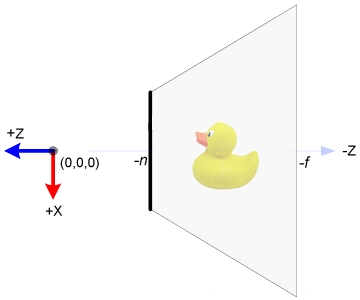
\includegraphics[width=0.45\linewidth,keepaspectratio=true]{figs/scene01.png}
&
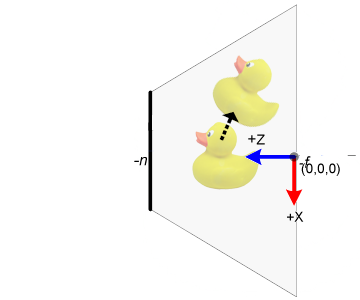
\includegraphics[width=0.45\linewidth,keepaspectratio=true]{figs/scene02.png}
\\
(a)&(b)\\ \hline
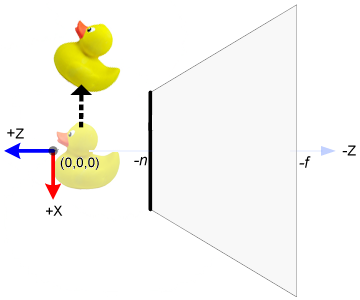
\includegraphics[width=0.45\linewidth,keepaspectratio=true]{figs/scene03.png}
&
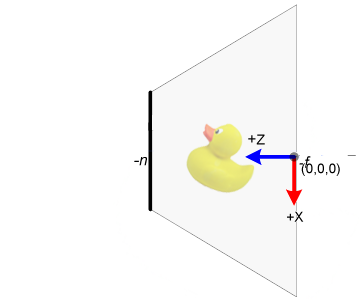
\includegraphics[width=0.45\linewidth,keepaspectratio=true]{figs/scene04.png}
\\ 
(c)&(d)\\ \hline
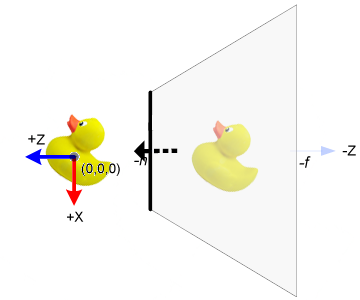
\includegraphics[width=0.45\linewidth,keepaspectratio=true]{figs/scene05.png}
&
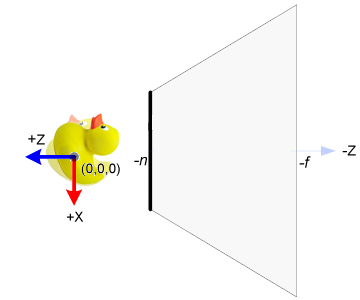
\includegraphics[width=0.45\linewidth,keepaspectratio=true]{figs/scene06.png}
\\ 
(e)&(f)\\ \hline
\end{tabular}
\caption{Example of a scene composed by a duck and the projection frustum defined by the near and far planes, respectively $n$ and $f$. The viewer is at left center in pictures (a) and (b) and in the top left corner in pictures (c) to (f).}
\label{fig.transformation}
\end{figure}




